\documentclass[a4paper]{article}
\usepackage[T1]{fontenc}
\usepackage[utf8]{inputenc}
\usepackage[swedish]{babel}
\usepackage{verbatim}
\usepackage{hyperref}
\usepackage{fancyvrb}
\usepackage{listings}
\usepackage[pdftex]{graphicx}
\fvset{tabsize=4}
\fvset{fontsize=\small}

\newif\ifpdf
\ifx\pdfoutput\undefined
  \psffalse
\else
  \pdftrue
\fi
\ifpdf
  \usepackage[pdftex]{graphics}
\else
  \usepackage{graphics}
\fi

\title{Guitar tuner \\ Digitala Projekt (EITF40)}
\author{\\Jakub Gorski, D07 (dt07jg8@student.lth.se)\\
Patrik Thoresson, D07 (dt07pt2@student.lth.se)\\\\Handledare: Bertil Lindvall}
\date{Inlämnad: 2011-03-01}


\begin{document}


\maketitle
\thispagestyle{empty}

\begin{abstract}
This project focuses on constructing a guitar tuner with an \texttt{ATmega16}. The tuner will be able to tune any instrument that can be connected to the tuner using a $3.5mm$ analog jack. The difference between this tuner and other tuners is that it will use the \texttt{ATmega16}’s internal \textit{ADC} to measure the frequencies, whereas others usually use \textit{Voltage-Controlled Oscillators}.
\end{abstract}


\newpage
\thispagestyle{empty}
\tableofcontents
\newpage
\pagenumbering{arabic}



\section{Inledning}
Detta projekt var en del av kursen \textit{Digitala och Analoga Projekt}, \texttt{EITF40}, på Lunds Tekniska Högskola. Som projekt konstruerades en stämapparat. Syftet med projektet är att skaffa sig ett klart koncept av det man vill konstruera, samtidigt som man behåller utrymme för eventuell vidareutveckling. I detta fallet kommer vidareutvecklingen att anspela på \texttt{ATmega16}:s \textit{ADC}\footnote{Analog-to-Digital Converter} som även i fortsättningen kommer möjliggöra en eventuell förvrängning av insignalen som kommer ge stämapparaten möjligheten att även vara en enklare effektprocessor. Resultatet blev en fungerande kromatisk stämapparat som automatiskt detekterar aktuell sträng, varpå den indikerar dess felmarginal och låter användaren stämma gitarren.

\section{Kravspecifikation}
Syftet med kravspecifikationen var att i ett tidigt stadium bestämma vilka funktioner stämapparaten bör hantera.
\subsection{Ursprunglig kravspecifikation}
\begin{itemize}
\item Kretsen ska kunna användas som en stämapparat, där 7 lysdioder indikerar huruvida instrumentet är stämt i förhållande till önskad frekvens.
\item Instrumentet kommer att anslutas via en 3.5mm mono \textit{TRS}-anslutning.
\item När kretsen inte är använd efter 1 minut kommer den att gå in i ett standby läge.
\item Ljudet från en gitarr ska kunna förvrängas till olika förbestämda effekter.
\item För att kunna skifta mellan effekter används knappar varpå information kommer att visas på LCD displayen.
\end{itemize}

\subsection{Uppfyllda specifikationskrav}
Under projektets gång märktes det att kravspecifikationen var för ambitiös. Till en början skulle kretsen fungera som en stämapparat och om tiden räckte till skulle gitarreffekter, samt övriga funktionskrav läggas till. Därför lades fokus på de grundläggande funktionerna som en fungerande stämapparat kräver. Inom dessa krav hamnade bland annat signalförstärkning och lysdioder som indikerar strängens felmarginal. Den slutgiltiga stämapparaten uppfyllde följande krav:

\begin{itemize}
\item Kretsen ska kunna användas som en stämapparat, där 7 lysdioder indikerar huruvida instrumentet är stämt i förhållande till den önskade frekvensen.
\item Instrumentet kommer att anslutas via on 3.5mm mono \textit{TRS} anslutning.
\item Tonens felmarginal skall visualiseras med hjälp av 7 lysdioder.
\end{itemize}

%\begin{figure}[!h]
%\begin{center}
%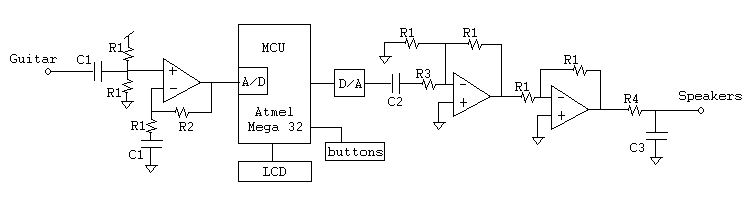
\includegraphics[scale=0.5]{circuit.png}
%\caption{En guitar fx DSP processor på en Atmega32.}
%\label{FBG_proterties}
%\end{center}
%\end{figure}

\section{Konstruktion}
I vår slutgiltiga konstruktion använde vi oss av följande komponenter:
\begin{itemize}
\item 2x OP-förstärkare (\textit{CA3160E}).\cite{op}
\item \texttt{ATmega16}, 8-bit Mikrokontroller med 16KiB programmerbart minne.\cite{atmega16}
\item Analog to Digital Converter (\textit{ADC}) som är inbyggd i \texttt{ATmega16}.
\item 3x $10k$ trimpots.
\item $5k$ trimpot.
\item $1k$ trimpot.
\item $500k$ trimpot.
\item 2x $18pF$ kondensatorer.
\item 5x $4.7nF$ kondensatorer.
\item 1x \textit{898-3-R1K} motstånd.
\item 7x LED dioder. Varav 4x orange, 2x röda och 1x grön. Meddelar om strängens nuvarande avvikelse.
\item \textit{CMACKD} 8MHz kristall.
\item 2x $1k$ motstånd.
\item $10 \mu H$ spole.
\end{itemize}

\section{Metod}
\subsection{Testkopplingar}
Inledningsvis användes ett testbräde för att testa att OP-förstärkaren fungerade som tänkt. Kopplingen ritades upp och kopplades sedan enligt vår design. En mikrofon användes till en början för att testa förstärkningen. Däremot så krävde en mikrofon en annorlunda krets för att fungera med den förstärkning vi tänkt oss. Målet var att förstärka signalen så att vågen täcker intervallet 0-2.5V på oscilloskopet, vilket bör ge en amplitud på $2.5V$. Denna amplitud på insignalen är eftertraktad då \texttt{ATmega16}:s \textit{ADC} har en intern referensspänning på $2.56V$, vilket resulterar i en 8-bitars upplösning på samplingen då \textit{ADC}:ns interna förstärkning är avstängd.\cite[p.~205]{atmega16}

Med denna lösning syntes endast topparna av ljudvågen på oscilloskopet, vilket också tydde på att enbart den positiva halvan av vågen förstärks. Detta på grund av att OP-förstärkaren var jordad och kunde därmed inte förstärka den negativa delen av insignalen. Genom att införa en spänningsdelare mellan mikrofonen och OP-förstärkaren åtgärdades detta. Därmed förstärktes spännings-differensen mellan ingångarna på OP:n, vilket gjorde att utspänningen var $1.25V$ när insignalens spänning var $0V$. Den fullständiga, förstärkta vågen, kunde därefter representeras på oscilloskopet med intervallet $0-1.25V$, för dess negativa amplitud samt $1.25$-$2.5V$ för den positiva delen av vågen.

\subsection{Insignal och förstärkning}
Eftersom mikrofonen endast användes i testsyften byttes den i detta stadiet ut till förmån av en $3.5mm$ \textit{TRS}-anslutning där en gitarr kopplades in. I denna delen av projektet påbörjades även försök att sampla signalen i programkod, vilket medförde att en $8MHz$ kristall kopplades in tillsammans med två stycken $18nF$ kondensatorer\cite{hw} för att accelerera kristallen vid uppstart av \texttt{ATmega}:n.\cite{oscillator}

Spänningsdelaren, som justerar spännings-differensen på ovannämnda OP-förstärkare, reglerades av två stycken variabla resistorer, vars inställning gav den önskade utsignalen. Däremot visade det sig vara svårt att kalibrera spänningsdelaren. Detta medförde att en tongenerator användes för att få så exakt ton som möjligt, varpå OP:ns variabla resistorer justerades med assistans av oscilloskop. Efter kalibreringen av OP-förstärkaren blev det uppenbart att insignalens förstärkning, som då var på $500x$, var otillräcklig. Testerna visade att en ytterligare en förstärkare behövdes för att insignalen till \textit{ADC}:n skulle ha tillräcklig amplitud för att kunna detektera ljudvågen. Dessutom kunde denna förstärkning inte höjas ytterligare utan att drabbas av internt brus, därför infördes en extra OP-förstärkare som kopplades i serie för att nå en maximal amplitud på $2.5V$.\cite{op}

Sammanfattningsvis, vågen som enligt oscilloskopet endast innehar en positiv amplitud, justeras genom förstärkning av spännings-differensen, till att hela signalen kunde ses inom intervallet $0$-$2.5V$ på oscilloskopet. Detta medförde också att eventuell tystnad på ingången till stämapparaten gav en $1.25V$ signal på oscilloskopet om den mäts efter de två förstärkarna.


\subsection{Hantering av brus}
\label{sec:brus}
När förstärkarna var på plats noterades det brus på insignalen till \textit{ADC}:n, vilket påverkade dess mätvärden. För att förebygga detta infördes lågpassfilter med kondensatorer på $4.7nF$ parallellt mellan samtliga strömingångar på komponenterna, samt en spole före $A_{vcc}$. Detta för att, enligt \texttt{ATmega16}-manualen, uppnå \textit{ADC} \textit{noise cancellation}.\cite[p.~210]{atmega16} Även efter dessa modifikationer syntes brus på oscilloskopet. Bruset låg på $1.25V$ på grund av den förstärkta spännings-differensen, varpå \textit{ADC}:n samplade brus. För att undvika sampling av brus ökades förstäkningen av signalen, medan spännings-differensen minskades.\cite{hw}

Detta medförde att \textit{ADC}:n endast såg dalarna i den inkommande vågformen, vilket löste brusproblemen då dalarna i signalen var mindre bruspåverkade än topparna. Tack vare detta stannade bruset på en högre nivå, medan signalens, renare, förstärkta dalar syntes täckte $0$-$2.5V$ intervallet. Men även detta orsakade problem, då det krävde en väldigt sträng tröskel i programkoden för registrerering av perioder, vilket orsakade dåliga mätvärden för frekvensen. Anledningen till problemet var att tidsräkningen i \texttt{TCNT1} påverkades av bruset, vilket medförde att den mätte felaktig tidsåtgång och därmed frekvens. Detta löstes genom att byta ut $4.7nF$ kondensatorn efter $3.5mm$ anslutningen i första OP-förstärkaren till en ny kondensator, varpå bruset försvann.

När förstärkarna ansågs vara tillräckligt bra på testbrädet, flyttades komponenterna till slutgiltiga kopplingsplattan och löddes till rätt pinnar på processorn.

\section{Mjukvara}
När förstäkningen av signalen var på en nivå att \textit{ADC}:n kunde registrera vågen påbörjades utvecklingen av mjukvaran. I detta skedet stämde mätvärdena både från oscilloskopet och \textit{ADC}:n överens. För att kunna beräkna antalet perioder behövdes det en effektiv metod av frekvensuppmätning. Detta löstes med hjälp av en timer \texttt{TCNT1} samt $62.500KHz$ samplingsfrekvens på \textit{ADC}:n.

\subsection{Timers}
Valet av \texttt{TCNT1} berodde på att \texttt{TCNT0} är en 8-bitars räknare och kunde därför endast räkna till 256, vilket orsakade overflow under samplingen som påverkade frekvensuträkningen. En 16-bitars räknare gav en mer exakt tidsuppmätning, vilket gav bättre mätvärden. \texttt{TCNT1} användes till en början med en prescaler på 64, vilket gjorde att den räknade upp varje gång klockan på processorn fullbordat 64 klockcykler. Eftersom \texttt{TCNT1} räknade för snabbt och gav upphov till overflow med en prescaler på 64, ändrades denna till 256 för att säkra dess tidsbuffert.

Overflow i \texttt{TCNT1} användes till en periodisk nollställning av frekvensuträknings-algoritmen, vilket inträffar automatiskt om en insignal inte påträffas under ungefär en sekund. Mer om detta i stycke \ref{sec:periodtröskel}.

\subsection{\textit{ADC} och sampling}
Samplingsfrekvensen för \textit{ADC}:n var satt till $62.500KHz$, vilket mostvarar en prescaler på 128. Valet av denna prescaler berodde på att en prescaler på 256 ger för låg sampling ifall signalen blir högfrekvent, medan en prescaler på, till exempel, 32 ger dålig precision, vilket medför att icke-existerande perioder, eller brus registreras. I detta skede representerades insignalen till \textit{ADC}:n på intervallet $0V$-$2.5V$ där spännings-differensen försköts så att endast undersidan av vågen hissades ner. 

För att samplingar skall kunna påbörjas automatiskt sattes \textit{ADC}:n i \textit{free running mode}, dock så var detta väldigt processorkrävande då processorn inväntade varje sampel, vilket orsakade stopp i exekveringen när \textit{ADC}:ns värde tilldelades till en variabel. För åtgärda detta sattes \texttt{ADIE} flaggan till 1 i \texttt{ADCSRA}, vilket gjorde att \textit{ADC}:n genererade ett avbrott för varje fullbordad sampel istället för att avbryta exekveringen.

Detta fungerade bra tills oscilloskopet påpekade brusproblem, vilket även påverkade frekvensuträkningen. Som ett försök att lösa problemet utökades \textit{ADC}:ns läge till \textit{ADC noise canceller}.\cite[p.~210]{atmega16} \textit{ADC}:ns \textit{free running mode} byttes ut mot läget \textit{single conversion mode}, samt så sattes processorn i viloläge före sampling programmets main-loop i syfte att minska digitalt brus.\cite[p.~219]{atmega16} Efter slutförd sampel sattes processorn igång igen genom att sätta \texttt{SE}-flaggan i \texttt{MCUR} till 1.

Även om denna metod minskade bruset, så minskade den även utrymmet för eventuell felsökning. Detta på grund av att den uppmätta signalen på oscilloskopet klipps av för var gång \texttt{ATmega16}:n går in i viloläge, vilket omöjliggör felsökning av insignalen. Även den effektiva samplingsfrekvensen minskas till hastigheten som processorn kan gå in respektive ut ur viloläget, vilket påverkar den digitala vågrepresentationen.

Trots ovannämnda åtgärder var bruset så pass stort att \textit{ADC}:n inte kunde mäta signalen. Det är även nämnvärt att både oscilloskop såsom \texttt{JTAG}:en påverkade \textit{ADC}:ns mätvärde när dessa var påkopplade. Mer om detta nämns i stycke \ref{sec:brus}.

Sammanfattningsvis, när brusfaktorn bedömdes vara ute ur bilden fortskred arbetet med syftet att optimera koden för frekvensuträkningen så att perioder registreras så korrekt som möjligt.

\subsection{Optimering av algoritm}

\subsubsection{Amplitud-tröskel}
Perioderna registrerades genom vänta tills \textit{ADC}:n påträffar lägsta tillståndet på vågen, varpå den markerar det som en period när vågen börjar stiga igen. För att undvika att brus skall registreras som perioder infördes ett minsta tröskelvärde som \texttt{ADCH} måste understiga (endast dalarna i sigalen mäts), vilket ger ett striktare villkor för när en period inträffar och ger bättre mätvärden.

En ytterligare kodoptimering kunde utföras genom att hoppa över de första fåtal perioder när en signal som når över tröskeln registreras. Tack vare detta införs det en variabel som först hoppar över ett konstant antal perioder före den riktiga frekvensmätningen, vilket ger insignalen tid att stabilisera.

\subsubsection{Period-tröskel}
\label{sec:periodtröskel}
Vid en beräkning med bristande antal registrerade perioder, inväntar algoritmen ytterligare perioder då användaren spelar på gitarren. Dödtiden mellan sista registrerade period och den tillkommande, när användaren spelar på strängen, räknades som en enda lång period.

Detta åtgärdades med \texttt{TCNT1}:s \textit{overflow interrupt} som via en avbrottsrutin, när räknaren gått förbi sitt maxvärde, nollställer algoritmens variabler.\cite[p.~114]{atmega16} Dock så hjälper inte detta om det kommer en insignal igen innan räknaren hunnit hamna i avbrottsrutinen. Därför infördes en variabel som håller reda på \texttt{TCNT1}:s förra värde, med vars hjälp man kan se när senaste perioden inträffat. På så sätt körs algoritmen om när tidsåtgången mellan två perioder är för stor, vilket tyder på att perioderna hör till två olika tillfällen då användaren spelat på gitarren.

\subsection{Omräkning av konstanter}

När rätt antal perioder har uppmätts, hämtas \texttt{TCNT1} som mäter tiden. För att underlätta uträkning av frekvensen räknades frekvensvärdena om. Varje ton som stämapparaten bör kunna detektera\cite{tunings}, omräknas från $Hz$ till ett \texttt{TCNT1}-värde enligt nedanstående formel. Detta på grund av att uträkning av frekvens krävde i vanliga fall en division, som kan undvikas om man vänder på problemet. Därför omräknades konstanterna som definierar toner, där divisionen utförs vid kompilering, istället för att utföra den varje gång.

\begin{eqnarray}
\label{eq:timer}
\frac{\frac{ prescaler_{TCNT1} }{ CPU_{freq} } \cdot n_{periods} }{ string_{Hz} } = TCNT1
\end{eqnarray}

\newpage


\begin{figure}[h]

\begin{verbatim}
          ------ 12804,777140335392762577228596646
          E      11377,42718446601941747572815534
          ------ 9950,077228596646072374227714034
          A      8522,7272727272727272727272727273
          ------ 7456,224596014672350550213145633
          D      6389,7219193020719738276990185387
          ------ 5587,419146666144194345454245896
          G      4785,1163740302164148632094732544
          ------ 4290,9463289234185913616225561635
          B      3796,7762838166207678600356390734
          ------ 3319,7040909683467696183137564675
          EH     2842,6318981200727713765918738629
          ------ 2365,5597052717987731348699912565			
\end{verbatim}

\caption{Övergångarna mellan strängar som värde av \texttt{TCNT1}}
\label{fig:timervärden}

\end{figure}

Efter denna konvertering kommer uträkningen motsvara värdet på \textit{TCNT1}. Samtliga divisioner i algoritmen är eliminerade.

\subsection{Tonläge}
När \texttt{TCNT1}:s värde är antaget sker identifiering av strängens tonläge. Identifieringen sker med hjälp av jämförelser av likhet med värdena i Figur \ref{fig:timervärden} som räknades ut enligt ekvation (\ref{eq:timer}). Jämförelserna består av tröskelövergångar mellan toner som räknas ut enligt:

\begin{eqnarray}
\frac{(tone_{adjacent\_LOW} - (tone_{adjacent\_HIGH} - tone_{adjacent\_LOW}))}{2} = TONE\ TRANSITION
\end{eqnarray}

Ekvationen stämmer förutom för den ljusaste tonövergången, då gäller följande:

\begin{eqnarray}
\frac{(tone_{E} + (tone_{E} - tone_{A}))}{2} = EH\_ETOP\ TRANSITION
\end{eqnarray}

Med hjälp av dessa konstanta övergångströsklar (även uträknade i Figur \ref{fig:timervärden}) kan resultatet visualiseras på \texttt{LED}-lamporna. Dock så krävs det mindre trösklar för övergångar mellan \texttt{LED}-lamporna. Detta sker i enlighet med:

\begin{eqnarray} %%FIXA
\frac{transition_{adjacent\_HIGH} - transition_{adjacent\_LOW}}{6} = LED\ OFFSET
\end{eqnarray}

Detta ser till att avvikelser från toner kan representeras visuellt med hjälp av \texttt{LED}-lamporna.

\section{Resultat}
Resultatet är en fungerande stämapparat med möjligheten att visa vilken avvikelse strängen har för tonen man stämmer mot. Den är inte särskilt exakt och har väldigt stränga tröskelvärden och villkor, vilket gör att man kan behöver spela på en sträng ett antal gånger innan signalen registreras som en godtyckligt stabiliserad våg. Insignalen kan fortfarande registreras fel om man råkar få in en oren ton. Till exempel om strängen man spelar på skorrar, eller om man råkar röra volymkontrollen på instrumentet man spelar på. Detta beror på att det bildas högfrekvent brus när man vrider på en potentiometer, på en gitarr likaså, som ytterligare förstärks med de två existerande OP-förstärkarna som används.

Stämapparaten har många variabla resistorer, varav tre reglerar förstärkningen, medan två reglerar spännings-differensen hos första OP-förstärkaren. Det är mycket som kan gå fel med så pass många trimpots, vilket det har gjort. För att kringgå högfrekventa bruset har bland annat spännings-differensen ökats så att endast den negativa delen av vågen syns på intervallet $0$-$2.5V$ vilket gav renare perioder. Mer om hur brusproblemen löstes nämns i \ref{sec:brus}.

\section{Slutsats}


I efterhand känns det som att vi inte borde använt testbrädet under så pass långt tid som vi faktiskt gjorde. Även om kretsen fungerade på testbrädet så skulle samma krets både se annorlunda ut och kopplas annorlunda vid lödning på kopplingsbrädet, vilket var tidskrävande. Vi skulle även kunnat använda oss av en \textit{Voltage-Controlled Oscillator}, vilket skulle dramatiskt minska kodkomplexiteten, men även förenkla hårdvaruimplementationen. Detta på grund av att en \textit{Voltage-Controlled-Oscillator} skickar en impuls varje gång en period inträffar i en signal, vilket förenklar frekvensuträkning. Dock så skulle detta begränsa eventuellt planerad funktionalitets-utökning. Projektet hade inte varit lika givande om det hade byggts med en \textit{Voltage-Controlled-Oscillator}.

Ständiga ändringar på förstärkarkonfigurationer med 5 variabla resistorer och nära samarbete med oscilloskop tog upp en större del av projektet. Implementationen av mjukvara tog drastiskt mindre tid. Detta har gett oss en bättre förståelse för hur en analog signal bör se ut för att den skall kunna digitaliseras.

\begin{thebibliography}{9}

\bibitem{atmega16}
  Datablad ATmega16,
 [online]
 Adress: <\url{http://www.eit.lth.se/fileadmin/eit/courses/edi021/datablad/Processors/ATmega16.pdf}>
 [Sista åtkomst 24 Februari 2011] 
 
\bibitem{op}
  Datablad OP-Amp CA3160.
 [online]
 Adress: <\url{http://www.eit.lth.se/fileadmin/eit/courses/edi021/datablad/Analog/opamp/ca3160.pdf}> 
 [Sista åtkomst 24 Februari 2011] 
 
 \bibitem{hw}
  USB and PIC Microprocessors 16C745 and 18F2455.
 [online]
 Från AlanMacek.com.
 Adress: <\url{http://www.alanmacek.com/usb/#Project_Hardware}>
 [Sista åtkomst 24 Februari 2011] 
 
 \bibitem{tunings}
  WA's Encyclopedia of Alternate Guitar Tunings.
 [online]
 Adress: <\url{http://members.cox.net/waguitartunings/tunings.htm}>
 [Sista åtkomst 24 Februari 2011] 
 
 \bibitem{oscillator}
 Reference Oscillator Crystal Requirements for the MC1320x, MC1321x, MC1322x, and MC1323x IEEE 802.15.4 Devices.
 [online]
 Freescale Semiconductor.
 Adress: <\url{http://cache.freescale.com/files/rf_if/doc/app_note/AN3251.pdf}>
 [Sista åtkomst 24 Februari 2011] 
\end{thebibliography}

\section{Appendix A - Källkod}
\lstset{tabsize=2, breaklines=true, basicstyle=\small\ttfamily, basewidth=0.51em}
\lstinputlisting{guitar_tuner.c}

\end{document}